\subsection{SIRS modelling}
	Here we confirmed that the recovery rate, $b$, should be smaller than the rate of transmission, $a$, to sustain a disease. We saw that there is a surprisingly good match between the RK4 and the MC model, but the MC model needs more time, approximately 3 years,  to stablize and find a steady - state in the population. Finally we figured that the MC simulation crashes if the number of infected people reaches zero. Details can be read below.
	
	The equilibrium expectation values and corresponding standard deviation, after 10 years of time or 3650 days, were found to be: \autocite{Nobody06}

\begin{table}[h]
\center
\begin{tabular}{llll}
      & S(t)   & I(t)   & R(t)   \\
Mean  & 108.81 & 110.11 & 181.06 \\
Stdev & 39.48  & 32.06  & 28.24  \\
\end{tabular}
\end{table}

	 
\subsubsection{4th order Runge-Kutta on the ODEs from SIRS, testing recovery rate.}
The simplest form of SIRS models differential equations solved with 4th order Runge - Kutta, then plottet. All plots in figure: \ref{fig:4RKSIRS}, have a black line that represent the change in total population. One can see there is not much change in population, as expected, at this moment. The equilibrium-states, discussed in section: \ref{sec:stady_state}, are plottet with stapled lines. These solutions are only plottet for one year, due to their obvious approach of the equilibrium-states. The difference between these figures are due to different recovery rate. One can see form these figures that after the initial burst of infection most develops an immunity after a short time and the disease reaches a steady-state. We can also confirm that if the transmission rate is larger then the recovery rate ($b<a$) the disease mange to get some kind of foothold, to sustain itself in the population.

\begin{figure}[H]
    \centering
    \begin{subfigure}{0.49\textwidth}
        \centering
        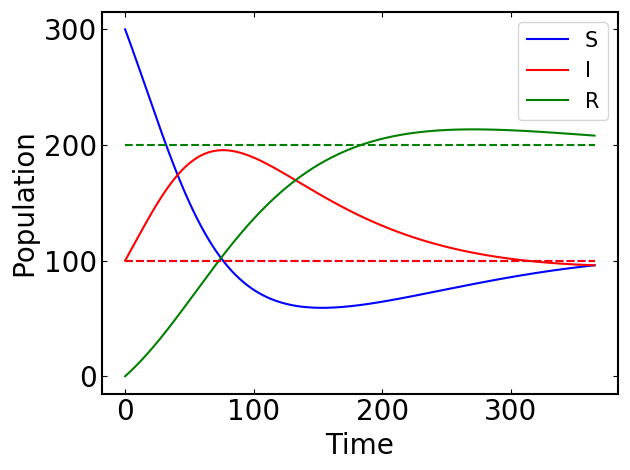
\includegraphics[width=\linewidth]{../fig/texfig/RK4_b1T1.png}
        \caption{Recovery rate, $b = 1$}
    \end{subfigure}%
     ~ 
    \begin{subfigure}{0.49\textwidth}
         \centering
         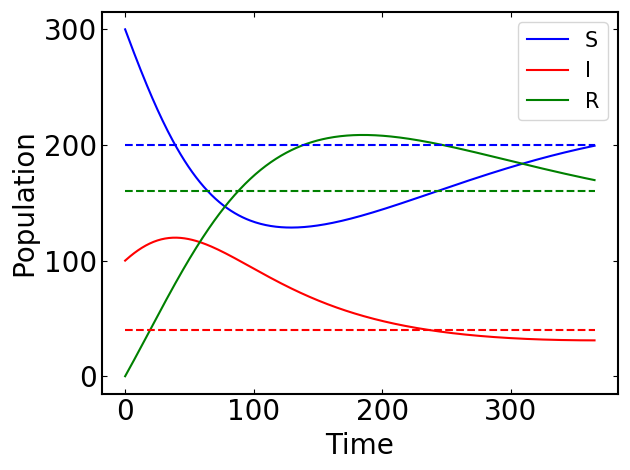
\includegraphics[width=\linewidth]{../fig/texfig/RK4_b2T1.png}
         \caption{Recovery rate, $b = 2$}
    \end{subfigure}
     ~ 
    \begin{subfigure}{0.49\textwidth}
         \centering
         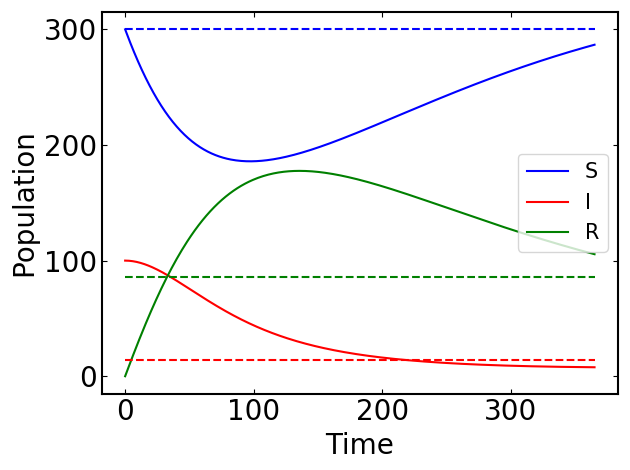
\includegraphics[width=\linewidth]{../fig/texfig/RK4_b3T1.png}
         \caption{Recovery rate, $b = 3$}
    \end{subfigure}
     ~ 
    \begin{subfigure}{0.49\textwidth}
         \centering
         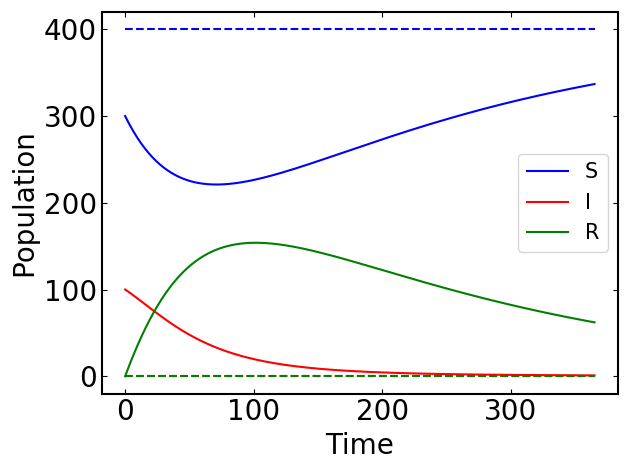
\includegraphics[width=\linewidth]{../fig/texfig/RK4_b4T1.png}
         \caption{Recovery rate, $b = 4$}
    \end{subfigure}
    \caption{4th order Runge-Kutta on ODEs given for SIRS model, where the only difference is the recovery rate,b, that is equal to $1,2,3,4$ respectivly}
    \label{fig:4RKSIRS}
\end{figure}

\subsubsection{Neural networks}





\subsubsection{Monte Carlo simulation of simple SIRS model, using different time.}
	Firstly we quickly understood that one year was simply not enough time to get to a proper stady-state, so we look at how the simulation would look if we ran it for $1,10,100,1000$ years. \ref{fig:MCb1Tchanges} And we quickly figured that $5$ to $10$ years should suffice, depending on what effects we want to observe. Here the both the equilibrium line, same as before, and the mean of the Monte Carlo simulation are plottet, and even after $1000$ years, these lines were still off by $1$ or $2$. 

\begin{figure}[H]
    \centering
    \begin{subfigure}{0.49\textwidth}
        \centering
        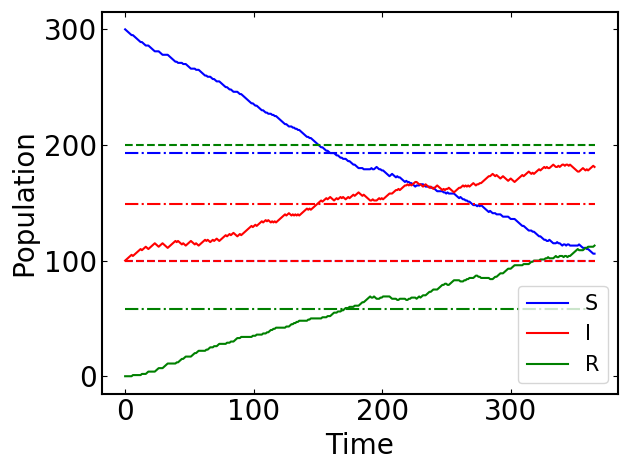
\includegraphics[width=\linewidth]{../fig/texfig/MC_T1.png}
        \caption{$T = 1$}
    \end{subfigure}%
     ~ 
    \begin{subfigure}{0.49\textwidth}
         \centering
         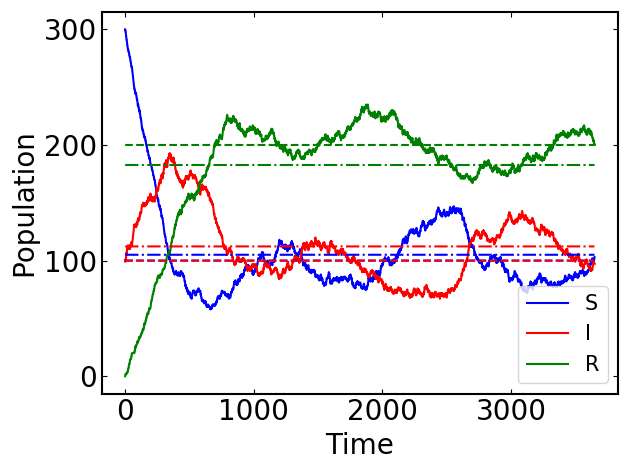
\includegraphics[width=\linewidth]{../fig/texfig/MC_T10.png}
         \caption{$T = 10$}
    \end{subfigure}
     ~ 
    \begin{subfigure}{0.49\textwidth}
         \centering
         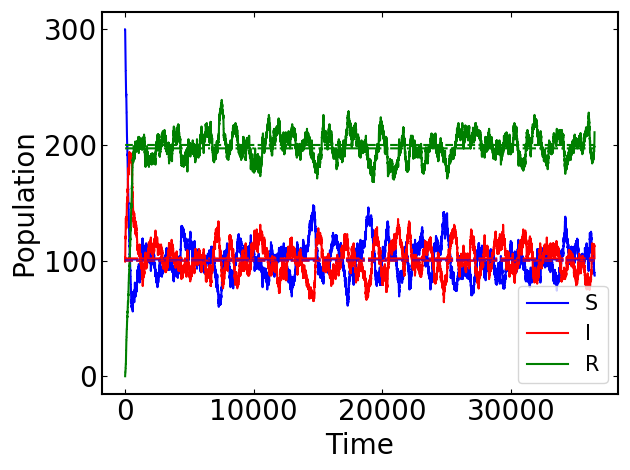
\includegraphics[width=\linewidth]{../fig/texfig/MC_T100.png}
         \caption{$T = 100$}
    \end{subfigure}
     ~ 
    \begin{subfigure}{0.49\textwidth}
         \centering
         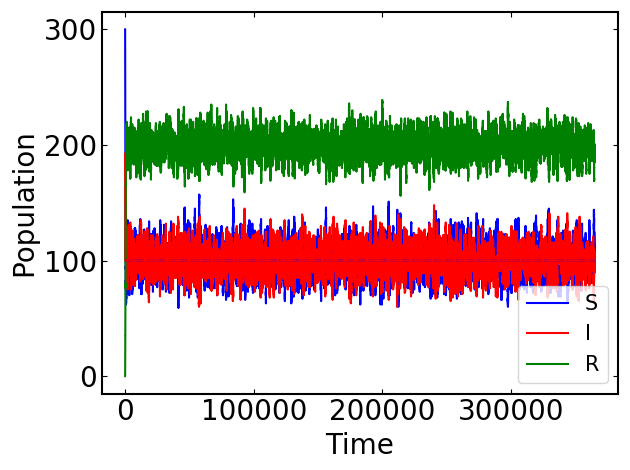
\includegraphics[width=\linewidth]{../fig/texfig/MC_T1000.png}
         \caption{$T = 1000$}
    \end{subfigure}
    \caption{Monte Carlo simulation of the simple SIRS model, the dotted lines are the equilibrium values and the dot-dashed lines are the mean of the functions. As we can see from the plot they vary }
    \label{fig:MCb1Tchanges}
\end{figure}

\subsubsection{Monte Carlo simulation of simple SIRS model, testing recovery rate}
	In these figures we notice something spectacular! The program crashes at higher recovery rate! This is due to the fact that there are no more infected people at some point in the program, and therefor no reason to track the infections development, if there is no infection. There are theoretical steady - state for the recovery rate,$b$,- values that are smaller then the transmission rate ,$a$, -values, but due to the randomness of the Monte Carlo Simulations the infection tend to die out by itself, which makes a lot of sense in a population that fluctuate. From here on out we will use $b=1$ in all figures. 
	 
\begin{figure}[H]
    \centering
    \begin{subfigure}{0.49\textwidth}
        \centering
        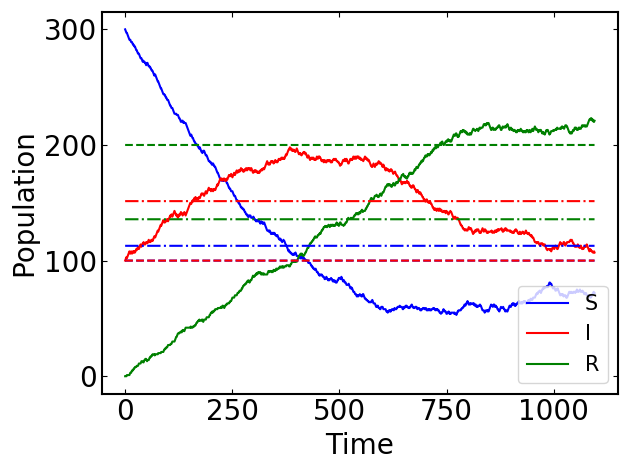
\includegraphics[width=\linewidth]{../fig/texfig/MC_b1T3.png}
        \caption{$T = 3$ and $b =1$}
    \end{subfigure}%
     ~ 
    \begin{subfigure}{0.49\textwidth}
         \centering
         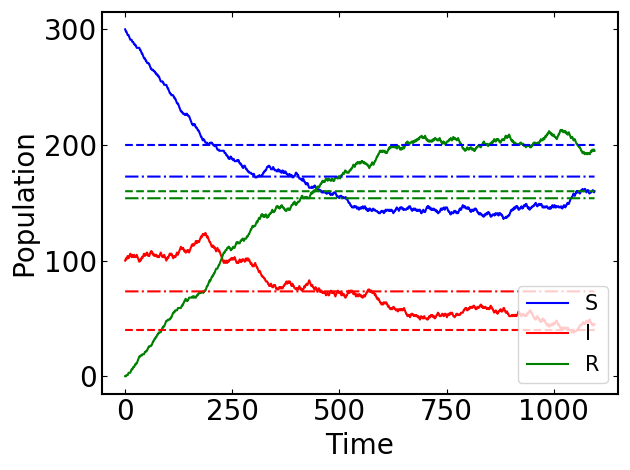
\includegraphics[width=\linewidth]{../fig/texfig/MC_b2T3.png}
         \caption{$T = 3$ and $b =2$}
    \end{subfigure}
     ~ 
    \begin{subfigure}{0.49\textwidth}
         \centering
         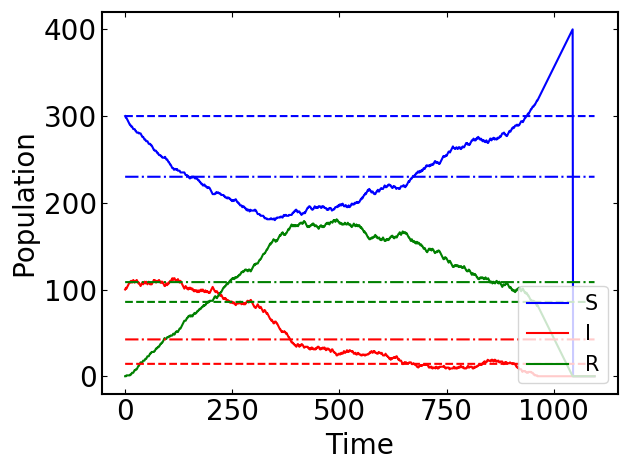
\includegraphics[width=\linewidth]{../fig/texfig/MC_b3T3.png}
         \caption{$T = 3$ and $b =3$}
    \end{subfigure}
     ~ 
    \begin{subfigure}{0.49\textwidth}
         \centering
         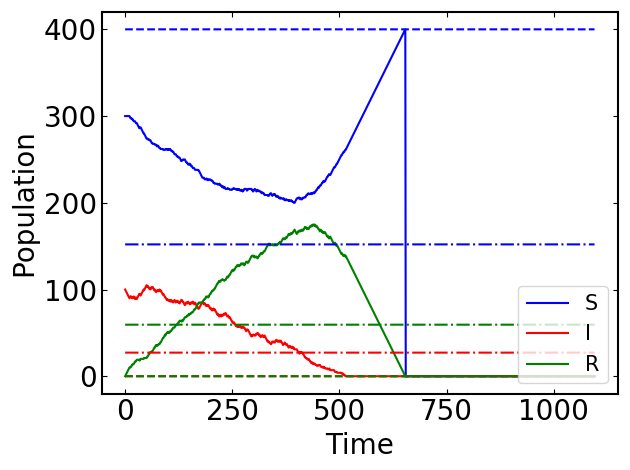
\includegraphics[width=\linewidth]{../fig/texfig/MC_b4T3.png}
         \caption{$T = 3$ and $b =4$ }
    \end{subfigure}
         ~ 
    \begin{subfigure}{0.6\textwidth}
         \centering
         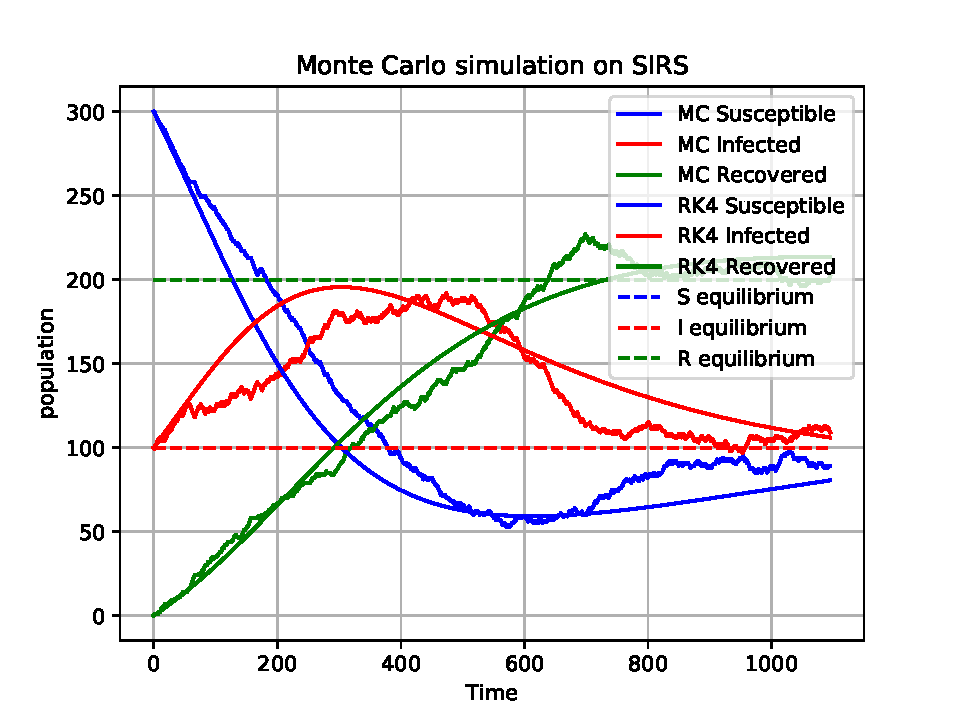
\includegraphics[width=\linewidth]{../fig/newfig/MCRK4_b1T3.pdf}
         \caption{$T = 3$ and $b =1$, both MC and RK4 plottet on top of each other.}
    \end{subfigure}
    \caption{}
    \label{fig:MCSIRS}
\end{figure}

\subsection{SIRS modelling with Improvements}
Here we present the results form the different versions of SIRS, Vital dynamics, Seasonal variation and Vaccination, and some of these combined. 

\subsubsection{Vital dynamics}
Vital dynamics are here included as presented in the theory section \ref{sec:VD} for both RK4 and MC. There is some difference in the given death/birth - rates between RK4 and MC due to lack of normalization $dt$. It is easy to see that these numbers are vital for both the survival and death of the disease

\begin{figure}[H]
    \centering
    \begin{subfigure}{0.49\textwidth}
        \centering
        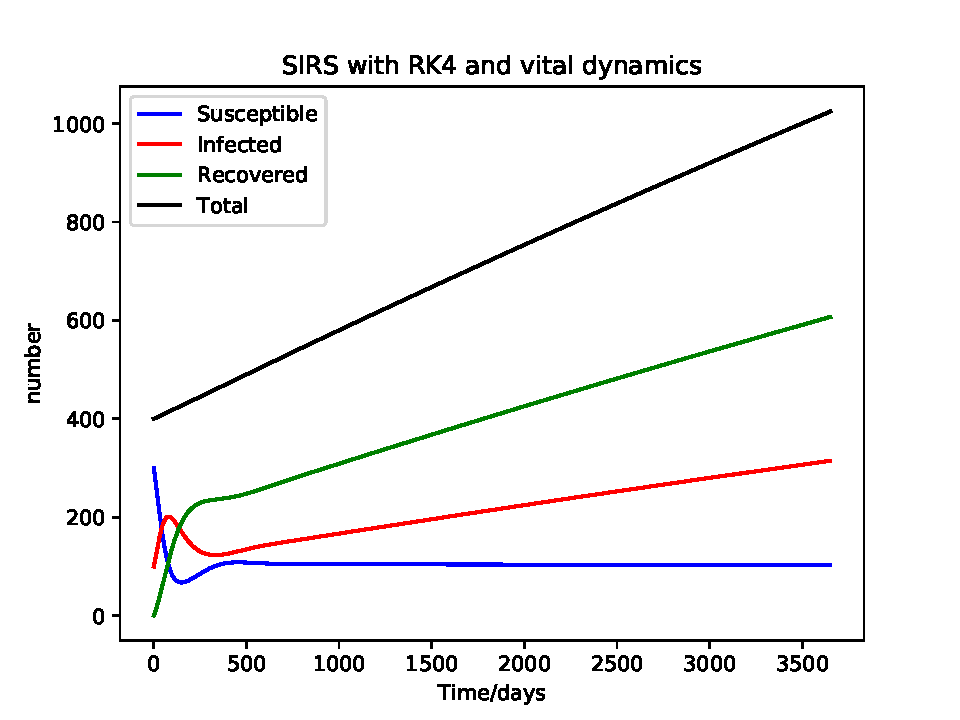
\includegraphics[width=\linewidth]{../fig/newfig/RK4_vitalDynamics_d001_dI01_e05.pdf}
        \caption{High birth-rate($e=0.05$), low death-rate, both in general, but also for the infected. ($d = 0.001, d_I =0.01$)}
    \end{subfigure}%
     ~ 
    \begin{subfigure}{0.49\textwidth}
         \centering
         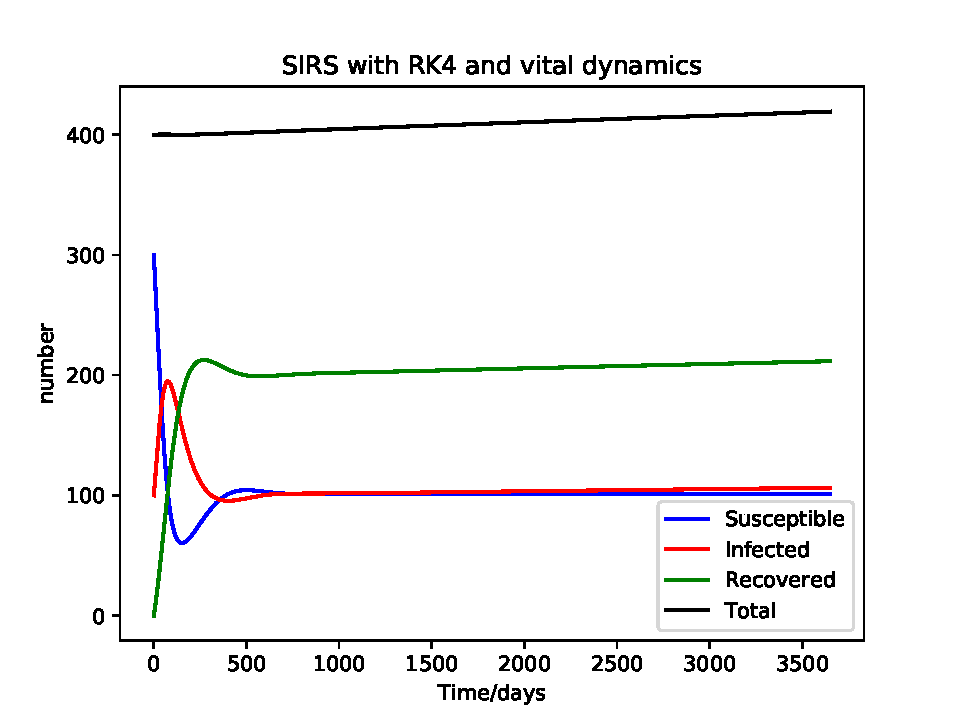
\includegraphics[width=\linewidth]{../fig/newfig/RK4_vitalDynamics_d001_dI01_e005.pdf}
         \caption{low birth-rate ($e = 0.005$), low death-rate, both in general, but also for the infected ($d = 0.001, d_I =0.01$)}
    \end{subfigure}
     ~ 
    \begin{subfigure}{0.49\textwidth}
         \centering
         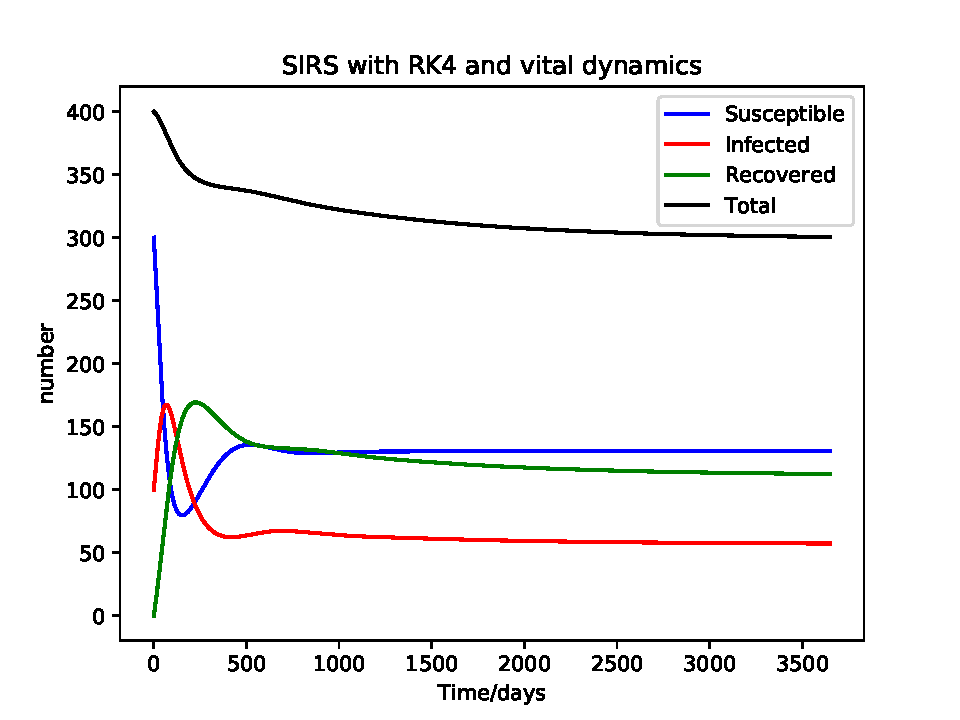
\includegraphics[width=\linewidth]{../fig/newfig/RK4_vitalDynamics_d01_dI30_e05.pdf}
         \caption{high birth-rate ($e=0.05$), high general death-rate and very high death-rate for the infected.}
    \end{subfigure}
     ~ 
    \begin{subfigure}{0.49\textwidth}
         \centering
         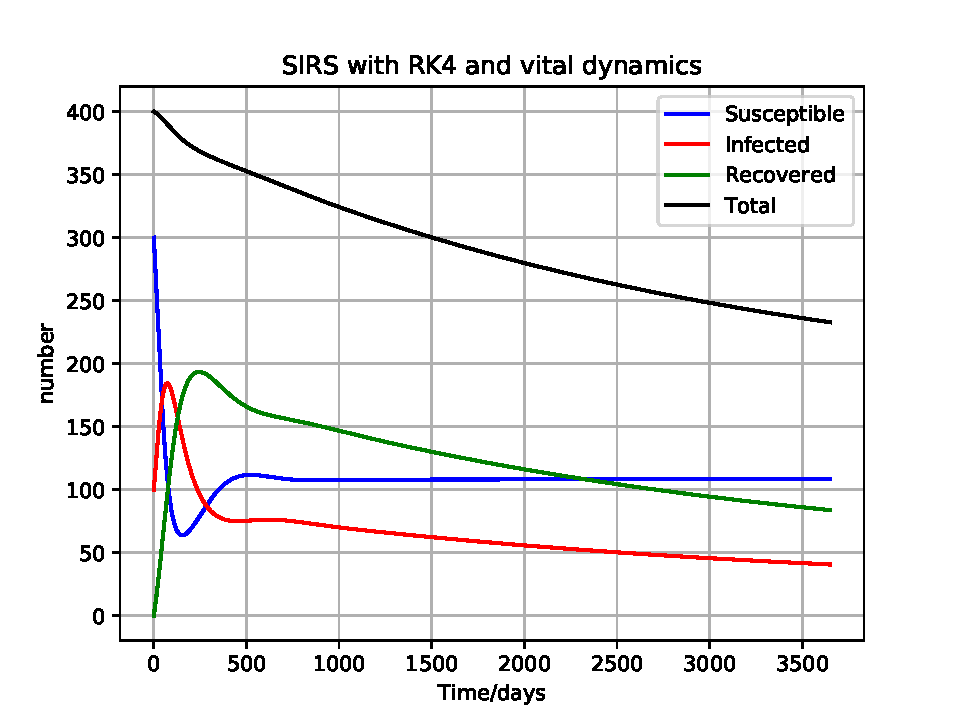
\includegraphics[width=\linewidth]{../fig/newfig/RK4_vitalDynamics_d002_dI10_e006.pdf}
         \caption{low birth-rate ($e=0.006$), low general death-rate($0.002$), high death-rate for infected($d_I = 0.10$)}
    \end{subfigure}
    \caption{Looking at different birth-, death-, infected death - rates.}
    \label{fig:RK4VD1}
\end{figure}


\begin{figure}[H]
    \centering
    \begin{subfigure}{0.49\textwidth}
        \centering
        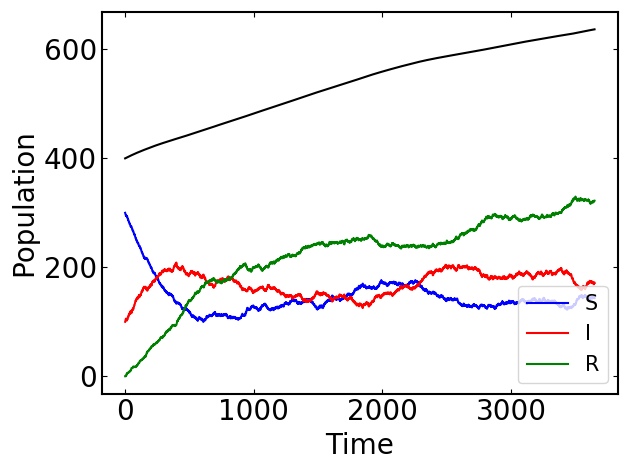
\includegraphics[width=\linewidth]{../fig/texfig/MC_vitaldynamic_d0002_dI0004_e0006.png}
        \caption{$d = 0.0002, d_I = 0.0004, e = 0.0006$}
    \end{subfigure}
     ~ 
    \begin{subfigure}{0.49\textwidth}
         \centering
         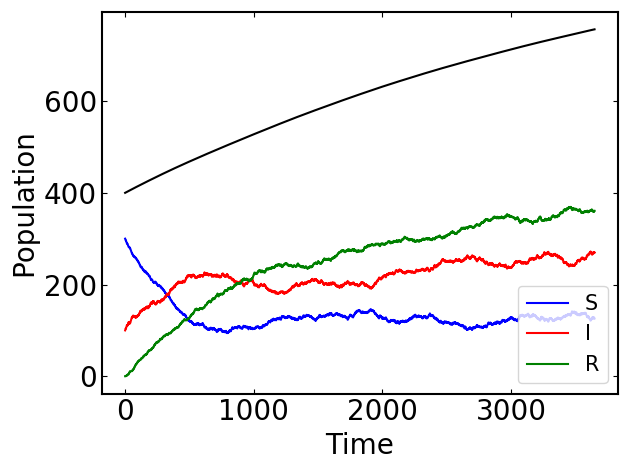
\includegraphics[width=\linewidth]{../fig/texfig/MC_vitaldynamic_d00002_dI0001_e00006.png}
         \caption{$d = 0.0002, d_I = 0.0001, e = 0.0006$}
    \end{subfigure}
     ~ 
    \begin{subfigure}{0.49\textwidth}
         \centering
         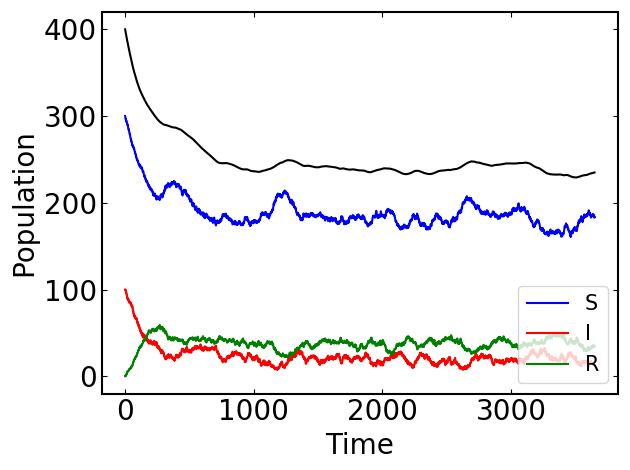
\includegraphics[width=\linewidth]{../fig/texfig/MC_vitaldynamic_d00002_dI001_e00006.png}
         \caption{$d = 0.0002, d_I = 0.001, e = 0.0006$}
    \end{subfigure}
     ~ 
    \begin{subfigure}{0.49\textwidth}
         \centering
         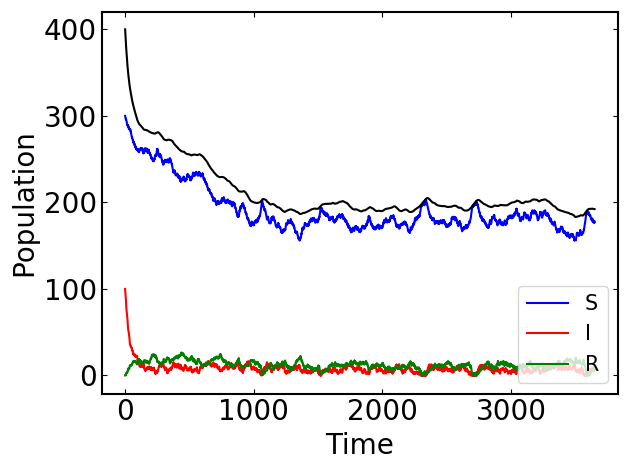
\includegraphics[width=\linewidth]{../fig/texfig/MC_vitaldynamic_d00002_dI003_e00006.png}
         \caption{$d = 0.0002, d_I = 0.03, e = 0.0006$}
    \end{subfigure}
    \caption{Main difference between the MC method and the RK4 is that $dt$ was not normalized in the cod, so smaller numbers had a much bigger impact.}
    \label{fig:RK4VD2}
\end{figure}


\pagebreak
\subsubsection{Seasonal Variation}
Here a Seasonal Variation is included \ref{sec:SV}, The value $A$ represents the maximum deviation from the infection rate $a_0=4$.  
\begin{figure}[H]
    \centering
    \begin{subfigure}{0.49\textwidth}
        \centering
        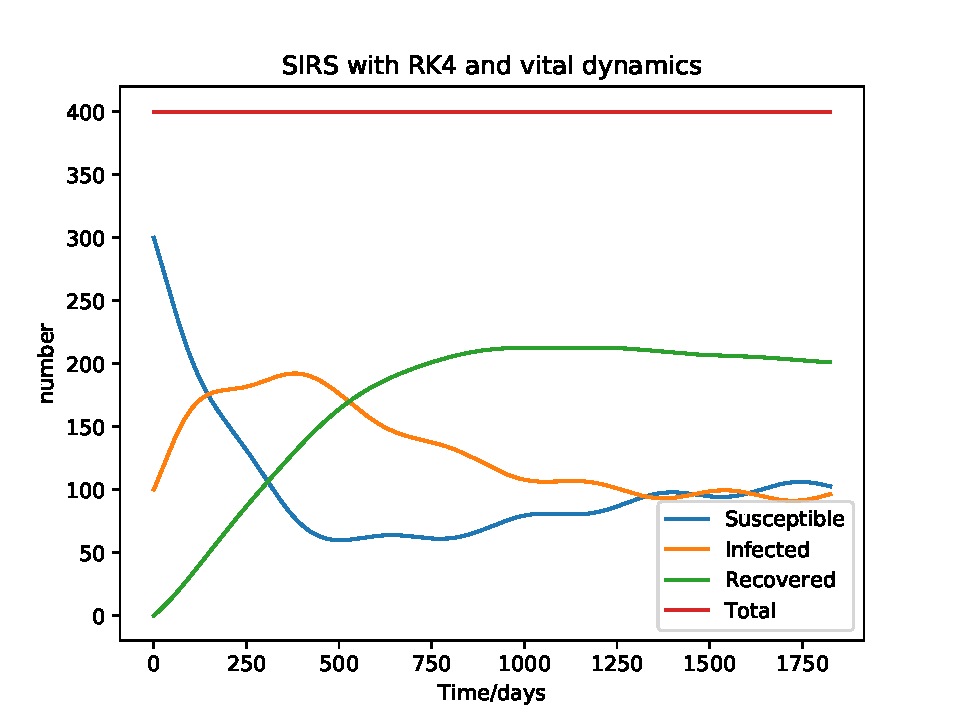
\includegraphics[width=\linewidth]{../fig/newfig/Vaccine_A=12_T=5.pdf}
        \caption{RK4 $A=1.2$}
    \end{subfigure}%
     ~ 
    \begin{subfigure}{0.49\textwidth}
         \centering
         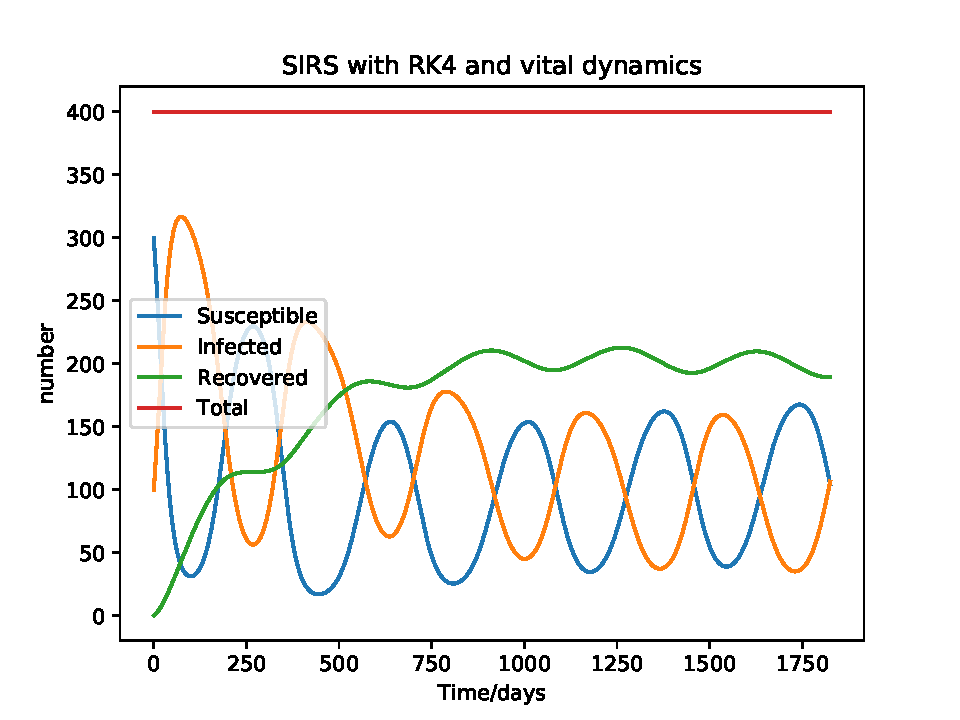
\includegraphics[width=\linewidth]{../fig/newfig/Vaccine_A=20_T=5.pdf}
         \caption{RK4$A=2.0$}
    \end{subfigure}
     ~ 
    \begin{subfigure}{0.49\textwidth}
         \centering
         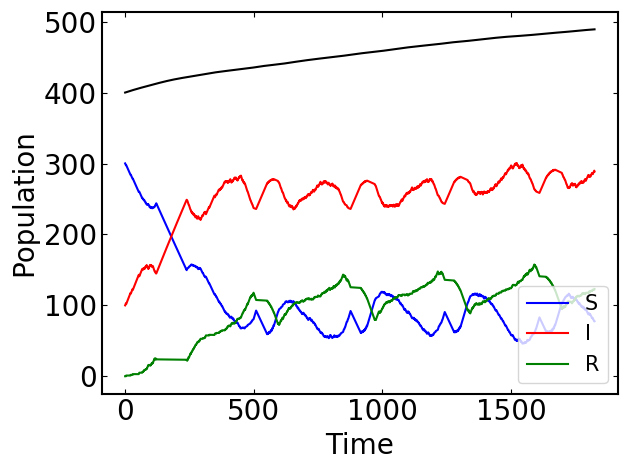
\includegraphics[width=\linewidth]{../fig/texfig/MCSV_A=12T=5.png}
         \caption{MC $A=12$ }
    \end{subfigure}
     ~ 
    \begin{subfigure}{0.49\textwidth}
         \centering
         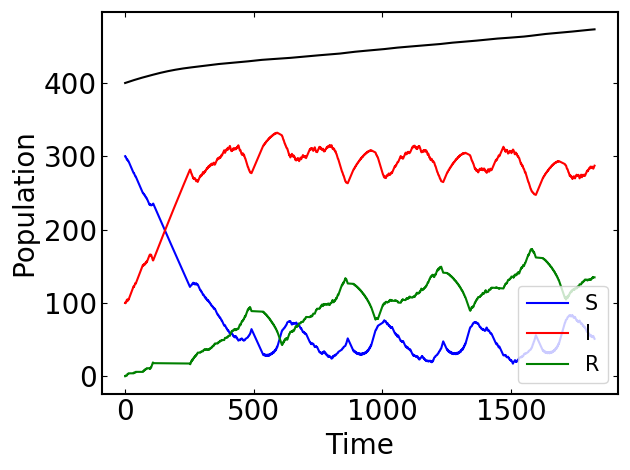
\includegraphics[width=\linewidth]{../fig/texfig/MCSV_A=20T=5.png}
         \caption{MC $A = 20$ }
    \end{subfigure}
    \caption{This figure shows the impact of seasonal variations on RK4 and MCS, notice how the seasonal variation impact is delayed in the MC scheme.}
    \label{fig:RK4VD3}
\end{figure}




\pagebreak
\subsubsection{Vaccination}
	If we assume that vaccines work and the earth is round, than we can see what incredible tool vaccines are for managing diseases. These results shows how efficient vaccine in combination with seasonal variation can be, when you only vaccinate $10\%$ of the population once per year.
\begin{figure}[H]
    \centering
    \begin{subfigure}{0.30\textwidth}
        \centering
        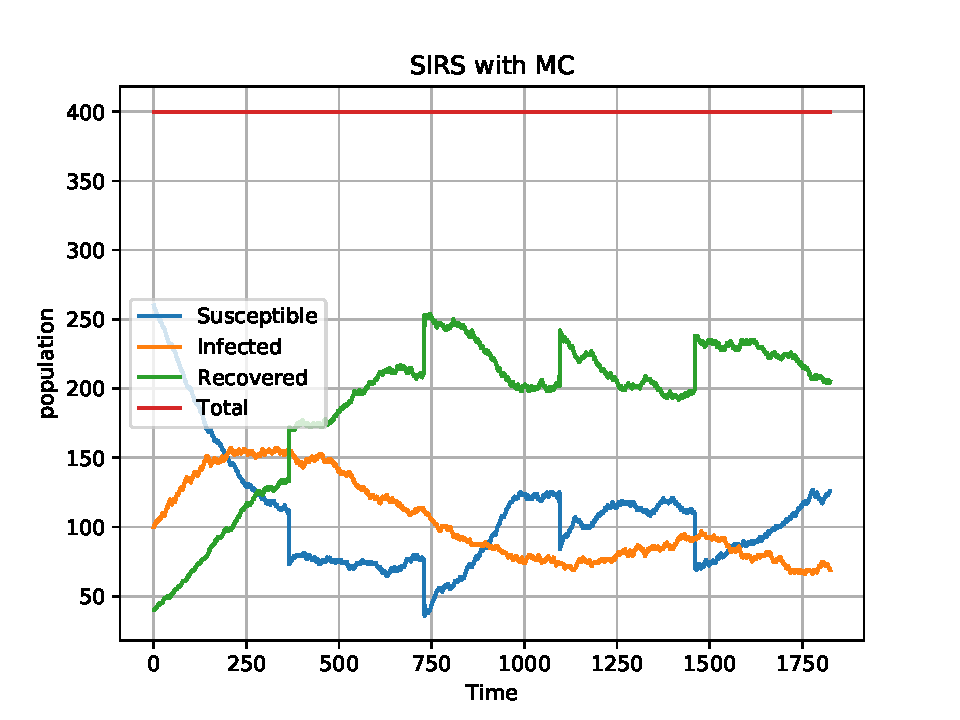
\includegraphics[width=\linewidth]{../fig/newfig/MC_onlyvaccineT=5f=40.pdf}
        \caption{MC vaccine}
    \end{subfigure}
     ~ 
    \begin{subfigure}{0.30\textwidth}
         \centering
         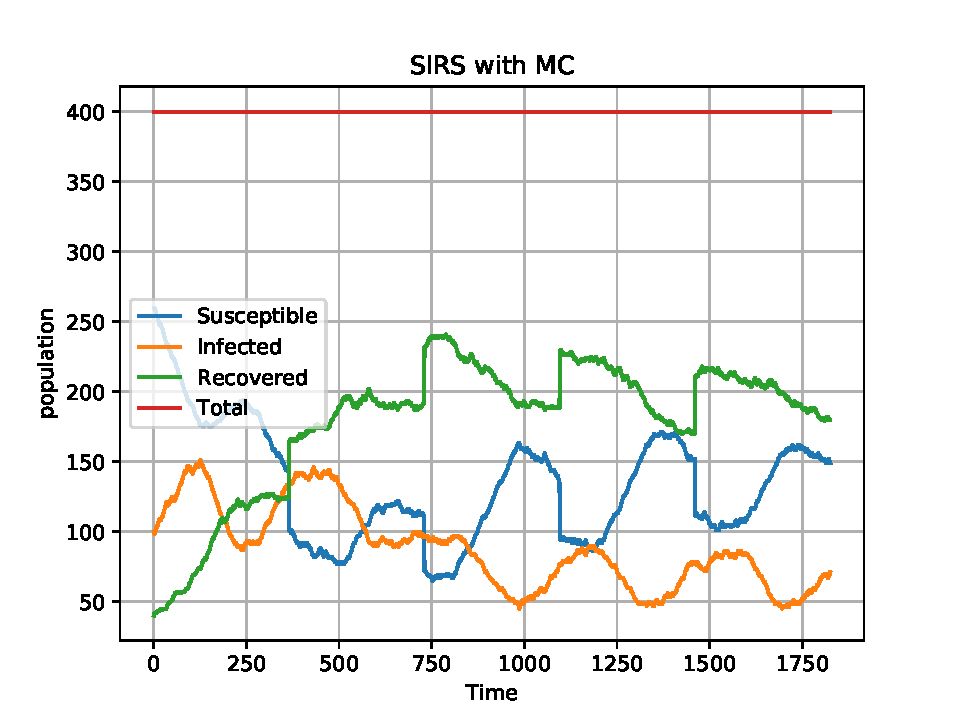
\includegraphics[width=\linewidth]{../fig/newfig/MC_vaccine_SVA=4_T=5f=40_notiming.pdf}
         \caption{MC vaccine no timing}
    \end{subfigure}
     ~ 
    \begin{subfigure}{0.30\textwidth}
         \centering
         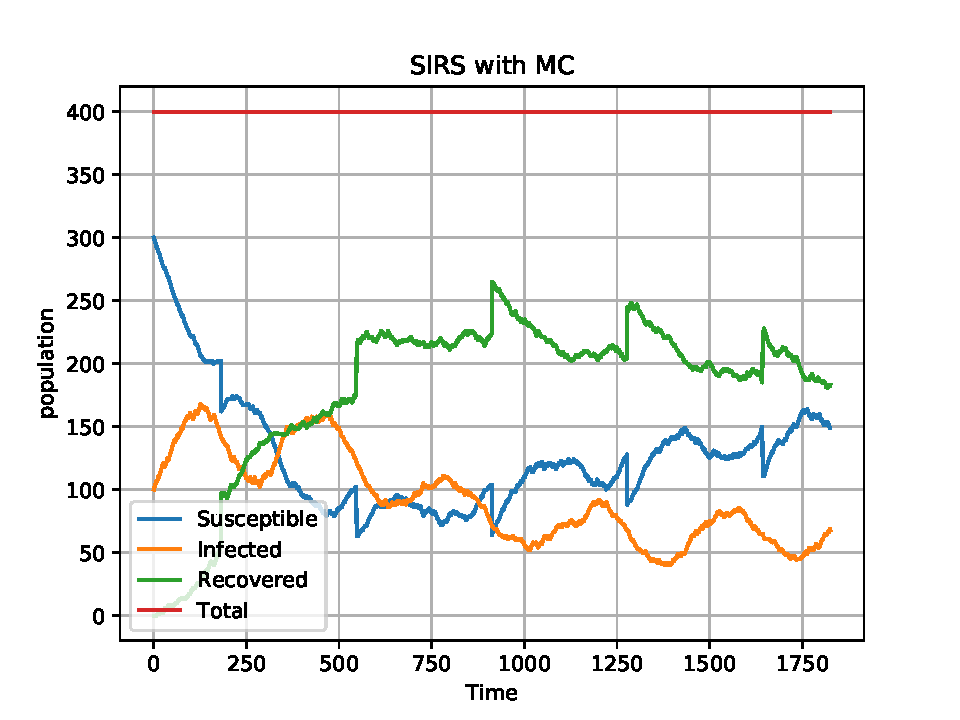
\includegraphics[width=\linewidth]{../fig/newfig/MC_vaccine_SVA=4_T=5f=40_timing.pdf}
         \caption{RK4 vaccine seasonal timing}
    \end{subfigure}
     ~ 
    \begin{subfigure}{0.30\textwidth}
         \centering
         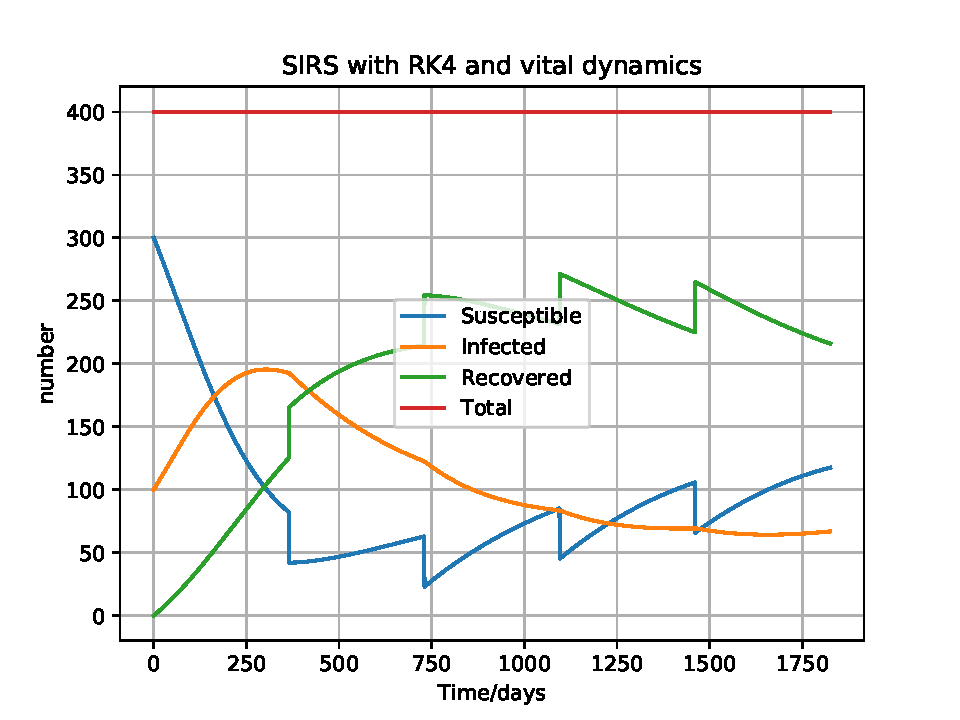
\includegraphics[width=\linewidth]{../fig/newfig/RK4Vaccine_f=40_T=5.pdf}
         \caption{RK4 vaccine}
    \end{subfigure}
     ~ 
    \begin{subfigure}{0.30\textwidth}
         \centering
         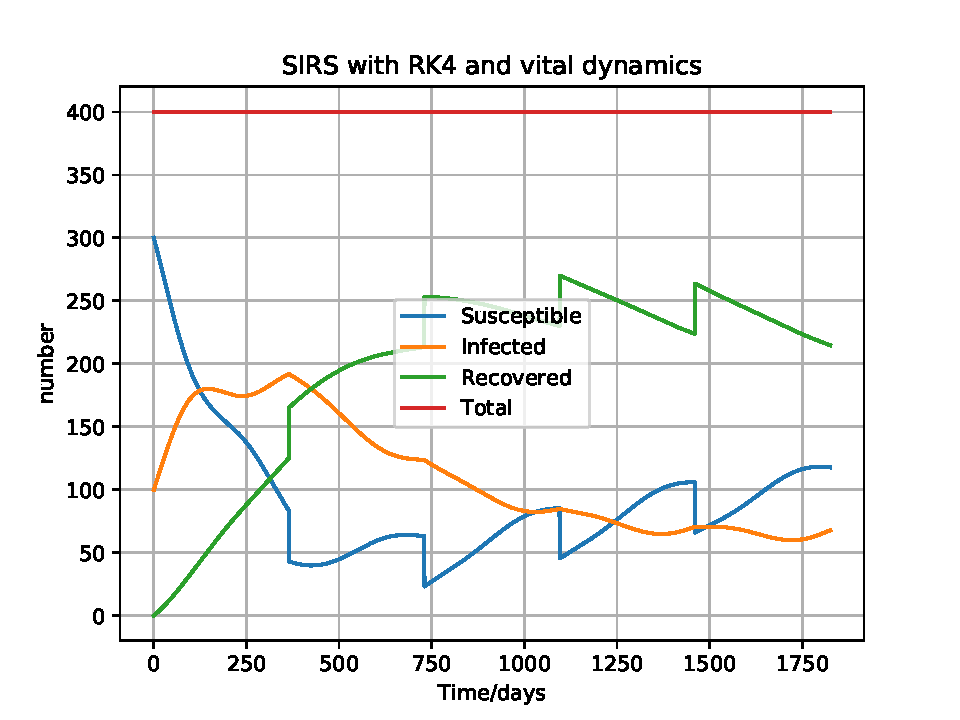
\includegraphics[width=\linewidth]{../fig/newfig/RK4Vaccine_SVA=2_f=40_T=5.pdf}
         \caption{RK4 vaccine no  timing}
    \end{subfigure}
     ~ 
    \begin{subfigure}{0.30\textwidth}
         \centering
         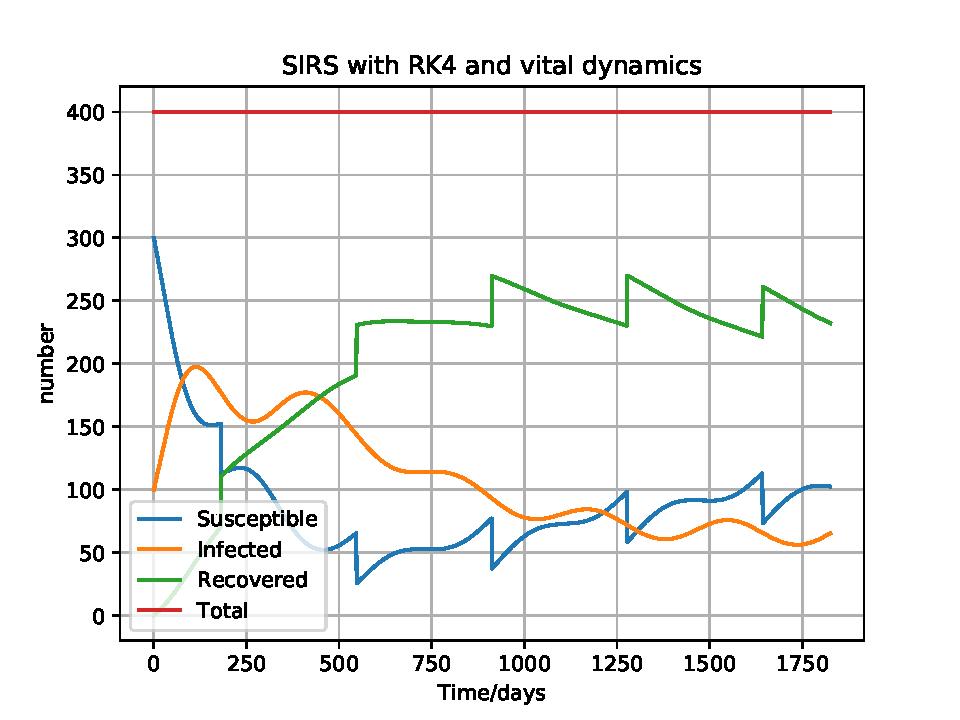
\includegraphics[width=\linewidth]{../fig/newfig/RK4Vaccine_SVA=4_f=40_T=5_timing.pdf}
         \caption{RK4 vaccine seasonal timing}
    \end{subfigure}
    \caption{The SIRS model, figure a) and d) are clean SIRS models with the effect of a yearly vaccine, b) and e) include the seasonal variation of the disease, lastly in figure c) and f) we have timed the vaccine to be given right before the winter, where it is assumed to be at its worst. (at least in this model).}
    \label{fig:MCVaccination}
\end{figure}




